\chapter{Implementación}

En este capítulo comentaremos a fondo las decisiones tomadas que hemos comentado previamente en base a la especificación, además de describir las implementaciones propuestas con las distintas tecnologías utilizadas. Pondremos el foco no solo en el \textbf{software implícito en el robot} sino también a los componentes desarrollados externos a él, pero que también conforman la arquitectura completa de la plataforma, como lo son el \textbf{sistema operativo}, el \textbf{panel web de administración} y otras herramientas involucradas. Las ideas que por una razón u otra no hayan llegado a implementarse a tiempo, serán definidas en profundidad en apartados posteriores.\\

Para elaborar este capítulo de una forma más legible y entendible, seguiremos una estructura muy similar a la propuesta en el capítulo 3 de \textbf{Especificación de requisitos}.\\


\section{Requisitos generales}


\subsection{Licencias y compartición del software}

En cuanto a licencias y permisos del proyecto, como se anticipó se usarán diversos \textbf{repositorios} en \textit{Github}, que aparecen listados a continuación y descritos en función del contenido (que se elaborará más tarde):

\begin{itemize}
	\item \textbf{\textit{lazarillo-embedded}} \cite{lazarillo-embedded}: se trata del software embebido programado en \textbf{\textit{C++}} que da lógica al robot.
	\item \textbf{\textit{lazarillo-admin-frontend}} \cite{lazarillo-admin-frontend}: es la página web que utilizan los técnicos para supervisar los robots y enviarles determinadas acciones. Se encuentra hecho en \textbf{\textit{React}} y utiliza \textit{WebSockets} para la conexión con el dispositivo.
	\item \textbf{\textit{lazarillo-admin-backend}} \cite{lazarillo-admin-backend}: es un servicio web que actúa como intermediario entre el robot y el servicio de \textbf{\textit{frontend}} para la negociación de la conexión. Está programado en \textbf{\textit{Python}} usando la librería de \textbf{\textit{Flask}} principalmente.
	\item \textbf{\textit{meta-lazarillo}} \cite{meta-lazarillo}: aquí se aloja el \textit{layer} (o ``capa'') personalizada para \textit{The Yocto Project} con la que se especifican las dependencias de \textbf{\textit{Lazarillo}} en la compilación del sistema operativo del robot.
	\item \textbf{\textit{documentacion-tfm}} \cite{documentacion-tfm}: en este repositorio se alojan los fuentes de \textbf{\LaTeX} para generar esta misma documentación que se está leyendo.
\end{itemize}

Todos los repositorios listados se publican bajo la licencia \textbf{\textit{GPL}} en su \textit{versión 3} (cuya última declaración es del 29 de junio de 2007 \cite{gplv3}) y que permite a cualquier interesado utilizar el software e incluso ampliar sus funcionalidades mientras que posteriormente se distribuya con la misma licencia.

Habiendo establecido ésto, entremos en materia y veamos todos los detalles de la implementación.\\


\section{Sistema operativo}

Como comentábamos en el capítulo del \textit{Estado del arte} en el apartado de \textit{Sistema operativo, el cerebro del robot}, existen diversas alternativas para componerlo. Partiendo de la base de que contamos con una \textit{Raspberry} como núcleo del computador, las opciones más sonadas son utilizar \textit{\textbf{Raspbian}} (sistema ya compilado e instalable en la plataforma) o crear nuestra propia distribución utilizando \textbf{el proyecto \textit{Yocto}}.\\

¿Por qué omitimos un sistema operativo que ya existe? Pues bien, la respuesta es fácil. \textit{Raspbian} es un sistema operativo de uso general que permite utilizar la \textit{Raspberry} como cualquier ordenador normal, ya sea para ofimática, desarrollo de software, consumo de recursos multimedia o incluso videojuegos. Esto provoca que el sistema operativo en cuestión venga con demasiado \textit{bloatware} (software innecesario que no se utiliza) preinstalado de base; y llevaría más tiempo modificar la imagen de \textit{Raspbian} para que no contenga todo el software no deseado que confeccionar un sistema operativo a medida. Además, deseamos que el robot solo muestre una aplicación embebida en pantalla en lugar de un entorno de escritorio normal, por lo que podemos prescindir de este entorno completo y configurar nuestro nuevo sistema para que solo muestre una aplicación y ahorre tiempo en el arranque.\\

La ventaja de crear nuestra propia imagen de sistema permitirá que incluyamos solo las librerías y dependencias que realmente necesitemos, obviando aspectos que no nos sea necesario incluir y que tomarían un espacio útil en la máquina. Además, siendo un proyecto de código abierto permitirá que interesados aprovechen el sistema operativo y lo extiendan con las funcionalidades y programas que les apetezca. Pasemos a continuación a comentar la implementación realizada.\\

\textbf{Nota}: este documento no se pretende que sea una guía de cómo utilizar \textit{Yocto} y entender todo su ecosistema, por lo que solo destacaremos las configuraciones personalizadas hechas para darle forma a \textbf{\textit{lazarillo-image}}.\\

Para empezar a trabajar con \textit{Yocto}, lo primero es elegir \textbf{la versión de \textit{Yocto}} a utilizar y seguir su documentación oficial sobre \textit{Quick Build} \cite{yocto-quick-build}, en la que se detalla cómo clonar el proyecto y realizar una primera compilación de prueba. Esta ejecución inicial llevará al menos un par de horas, ya que necesitará descargar todas las librerías necesarias y compilarlas.\\

\begin{figure}[h]
	\centering
	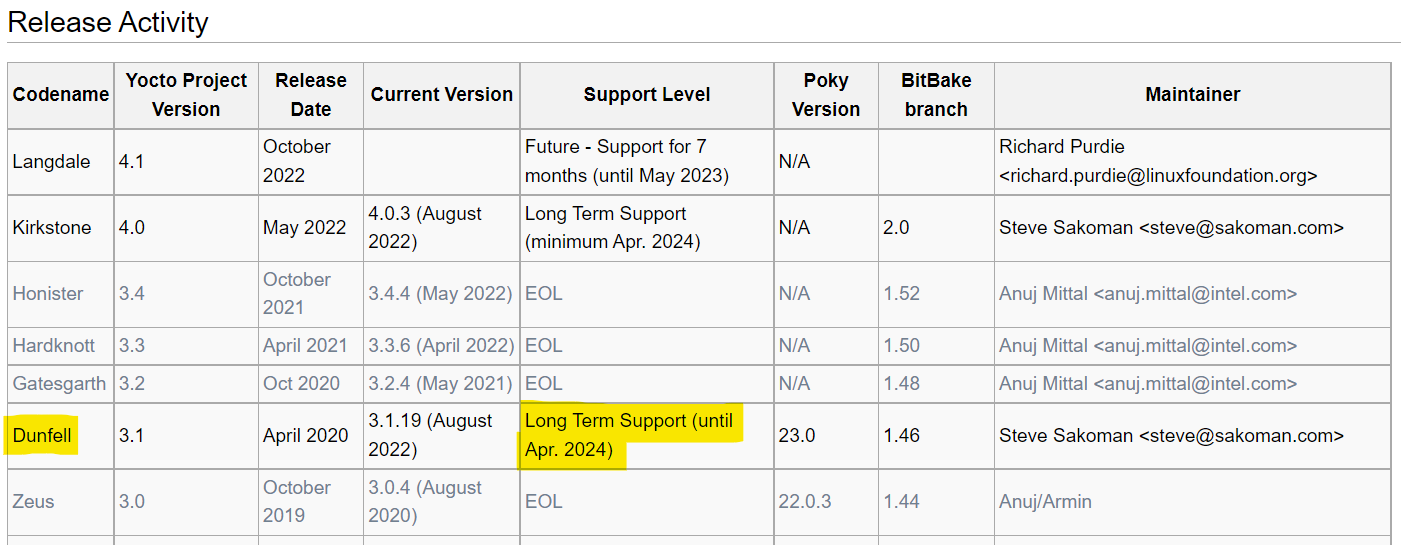
\includegraphics[width=0.85\textwidth]{imagenes/yocto-releases.png}
	\caption{La versión elegida es \textbf{\textit{Dunfell 3.1}} ya que lleva el suficiente tiempo en el mercado como para ser estable, y además es versión \textit{Long Term Support} y asegura soporte oficial hasta abril de 2024. Versiones más novedosas o no \textit{LTS} pueden no asegurar tanta estabilidad. - Fuente: \textit{Yocto Releases} \cite{yocto-releases}}
\end{figure}

Acto seguido, lo que hacemos para continuar con la creación de nuestra propia distribución son varias cosas:

\begin{itemize}
	\item Crear nuestro propio \textit{layer}, llamado \textbf{\textit{meta-lazarillo}} donde estableceremos nuestras directivas.
	\item Crear una \textbf{imagen} de sistema, que se llamará \textbf{\textit{lazarillo-image}} y que incluirá el software programado por nosotros y que se instalará automáticamente en el robot.
	\item Añadir a la imagen creada previamente las dependencias para que sus aplicaciones se ejecuten correctamente.
\end{itemize}

El contenido de este \textit{layer} puede verse en la web \cite{meta-lazarillo} pero igualmente listaremos aquí los archivos más representativos.\\

\subsubsection{conf/layer.conf}

Este primer archivo contiene las variables más genéricas para la configuración inicial del \textit{layer} y suele tener un formato parecido en todos los \textit{metas} que se crean, ya que principalmente fija el nombre característico de la colección además de la rama de \textbf{compatibilidad} (que es \textit{dunfell}) como hemos comentado arriba. 

\begin{lstlisting}
BBPATH .= ":${LAYERDIR}"

BBFILES += "${LAYERDIR}/recipes-*/*/*.bb \
${LAYERDIR}/recipes-*/*/*.bbappend"

BBFILE_COLLECTIONS += "lazarillo"
BBFILE_PATTERN_lazarillo = "^${LAYERDIR}/"
BBFILE_PRIORITY_lazarillo = "1"

LAYERSERIES_COMPAT_lazarillo = "dunfell"
LAYERVERSION_lazarillo = "1"
\end{lstlisting}


\subsubsection{recipes-core/images/lazarillo-image.bb}

A continuación, veamos el archivo que realmente define \textbf{la imagen} del sistema operativo, cuyo nombre utilizaremos cuando queramos compilarlo.

\begin{lstlisting}
inherit core-image lazarillo-class

GLIBC_GENERATE_LOCALES = "es_ES.UTF-8"

###################################################
# Groups of needed packages

CORE_PKGS = " \
	kernel-devicetree \
	kernel-image \
	kernel-modules \
	openssl \
"

MISC_PKGS = " \
	curl \
	nano \
	psplash \
"

QT_PKGS = " \
	qtbase qtbase-plugins qtbase-tools \
	qtdeclarative qtdeclarative-qmlplugins \
	qtgraphicaleffects qtgraphicaleffects-qmlplugins \
	qtmultimedia qtmultimedia qtmultimedia-plugins qtmultimedia-qmlplugins \
	qtquickcontrols qtquickcontrols-qmlplugins \
	qtquickcontrols2 qtquickcontrols2-qmlplugins \
	qtvirtualkeyboard qtvirtualkeyboard-plugins qtvirtualkeyboard-qmlplugins \
"

LAZARILLO_PKGS = " \
	lazarillo-embedded \
"

###################################################
# Installation of grouped packages

IMAGE_FEATURES += " \
	autologin \
"

IMAGE_INSTALL += " \
	${CORE_PKGS} \
	${MISC_PKGS} \
	${QT_PKGS} \
	${LAZARILLO_PKGS} \
"
\end{lstlisting}

Todas las constantes del tipo \emph{X\_PKGS} tan solo son valores auxiliares que se concatenan a \emph{IMAGE\_INSTALL} para que en la compilación se incluyan todas estas dependencias en el sistema de ficheros final.\\

Si nos fijamos en el valor de \emph{LAZARILLO\_PKGS} podemos ver que ahí se lista \textbf{lazarillo-embedded}, que se trata de la aplicación embebida que comentábamos que implementará toda nuestra lógica del robot. Vemos el contenido de su \textbf{receta} (como se llaman en \textit{Yocto} los archivos que definen cómo se debe obtener una pieza de software, compilarla e instalarla en el destino) en el siguiente apartado.\\


\subsubsection{recipes-core/lazarillo-embedded/lazarillo-embedded.bb}

\begin{lstlisting}
# Compiles Qt project with cmake after downloading
inherit cmake_qt5

# AUTOREV references to newest commit
SRCREV = "${AUTOREV}"
LICENSE = "GPLv3"

EXTRA_OECMAKE = "-DCOMPILE_MODE=d"

# Reference to repo where to download the software from
SRC_URI = "git://git@github.com/adrianmorente/lazarillo_hmi.git;protocol=ssh"

DEPENDS += " \
	qtbase \
	qtdeclarative \
	qtgraphicaleffects \
	qtmultimedia \
	qtquickcontrols \
	qtquickcontrols2 \
	qtvirtualkeyboard \
"

do_install() {
	install -d ${D}${bindir}
	install -m 0700 lazarillo-hmi ${D}${bindir}
	install -m 0700 motor-manager ${D}${bindir}
	install -m 0700 web-gateway ${D}${bindir}
}

FILES_${PN} = "${bindir}"
\end{lstlisting}

En el archivo mostrado se configura la \textit{URL} del repositorio del que \textit{Yocto} descargará el proyecto (usando las claves \textit{SSH} configuradas en el dispositivo de compilación).\\

Además, encontramos listadas las dependencias necesarias para la compilación exitosa del proyecto. Como utilizamos el framework \textit{Qt} en su versión \textbf{open source} (disponible en \cite{qt-open-source}) para construir la aplicación embebida, se enumeran las librerías que \textit{Yocto} deberá descargar e instalar también.\\

Para finalizar, con \emph{do\_install} establecemos que se copien al directorio normal de binarios del sistema operativo final (normalmente \emph{/usr/bin}) los tres programas generados por \emph{lazarillo-embedded}, con permisos de escritura, lectura y ejecución solo para el usuario actual. Por ahora nos ceñiremos a lo estrictamente relacionado con \textit{Yocto} y estos servicios los definiremos en detalle más adelante.\\


\subsubsection{Configuración local y compilación}

Una vez que tenemos nuestro \textit{layer} preparado para que \textbf{\textit{bitbake}}, la herramienta en \textit{Python} que gestiona las compilaciones de \textit{Yocto}, pueda encontrar nuestros paquetes y dependencias, pasamos a configurar el archivo \emph{build/conf/local.conf}, que es el realmente imprescindible. En este archivo podríamos haber añadido todo el contenido de configuración necesaria para compilar nuestra imagen, si bien es mucho más limpio utilizar \textit{layers} separados que poder versionar y controlar de forma independiente según la \textit{release} de \textit{Yocto} que queramos usar.\\

El contenido usado para el archivo es el siguiente (se han obviado algunas líneas por defecto de \textit{Yocto} que solo son para desarrollo y que no aportan mucho para el alcance de este documento):

\begin{lstlisting}
MACHINE = "raspberrypi3"

DISTRO = "poky"
DISTRO_FEATURES_append = " alsa alsa-plugins gles2 opengl pulseaudio systemd wifi"
DISTRO_FEATURES_REMOVE_append = " x11 wayland"
PACKAGECONFIG_pulseaudio += " systemd"
VIRTUAL-RUNTIME_init_manager = "systemd"
DISTRO_FEATURES_BACKFILL_CONSIDERED = "sysvinit"

PACKAGE_CLASSES = "package_deb"

BB_NUMBER_THREADS = "4"
PARALLEL_MAKE = "-j 4"

EXTRA_USERS_PARAMS += " usermod -a -G audio root;"
EXTRA_USERS_PARAMS += " usermod -P lazarillo123 root;"

EXTRA_IMAGE_FEATURES ?= "debug-tweaks"
\end{lstlisting}


En primer lugar, fijamos la \emph{MACHINE} de destino para la que queremos compilar, en este caso la \textit{Raspberry Pi 3} como hemos comentado anteriormente. Además, decimos a \textit{Yocto} que genere nuestra imagen de sistema operativo utilizando \emph{poky} como distribución base (que es la \textit{de facto} en la herramienta), además de añadir paquetes como \textit{Alsa}, \textit{Pulseaudio}, \textit{OpenGL} y \textit{Systemd}.\\

\begin{itemize}
	\item \textit{Alsa} y \textit{Pulseaudio} son dependencias para los sistemas de sonido, que aunque no se utilizan actualmente, se incluyen en el sistema para cuando se quieran emitir alertas sonoras a través del servicio \textbf{lazarillo-hmi} y así proporcionar una interfaz más cercana y accesible para los usuarios del robot.
	\item \textit{OpenGL} (y su complemento \textit{GLES2}) se incluyen ya que son requisitos indispensables para que el framework de \textit{Qt} con aplicaciones de interfaz gráfica funcione como esperamos en dispositivos embebidos. Gracias a esto, utilizamos el lenguaje \textit{QML} del framework (basado en \textit{Javascript}) para diseñar dicha aplicación con interfaz táctil.
	\item \textit{Systemd} se establece en el sistema como gestor de servicios y \textbf{demonios} (o \textit{daemons}, pequeños servicios que se ejecutan en segundo plano en el sistema). Este es el gestor de arranque de servicios por defecto en la mayoría de distribuciones modernas que utilizamos hoy en día para escritorio.
\end{itemize}

Para terminar, fijamos a \textit{Bitbake} que utilice 4 hilos en la compilación. Cuantos más se utilicen, más tareas de descarga/compilación/instalación podrán ejecutarse en paralelo. Obviamente dependerá de la máquina utilizada.\\

Para terminar, añadimos una contraseña al usuario \textit{root} por defecto para que no se pueda manipular libremente el robot por consola si se accede por \textit{ssh}.\\

Una vez tenemos listo nuestro \textit{layer} y el archivo \textit{local.conf}, podemos lanzar la orden \textbf{\textit{bitbake lazarillo-image}} en el directorio de desarrollo de \textit{Yocto} y ver cómo comienza a descargar dependencias y compilarlas en la arquitectura de la \textit{RPi}:

\begin{figure}[h]
	\centering
	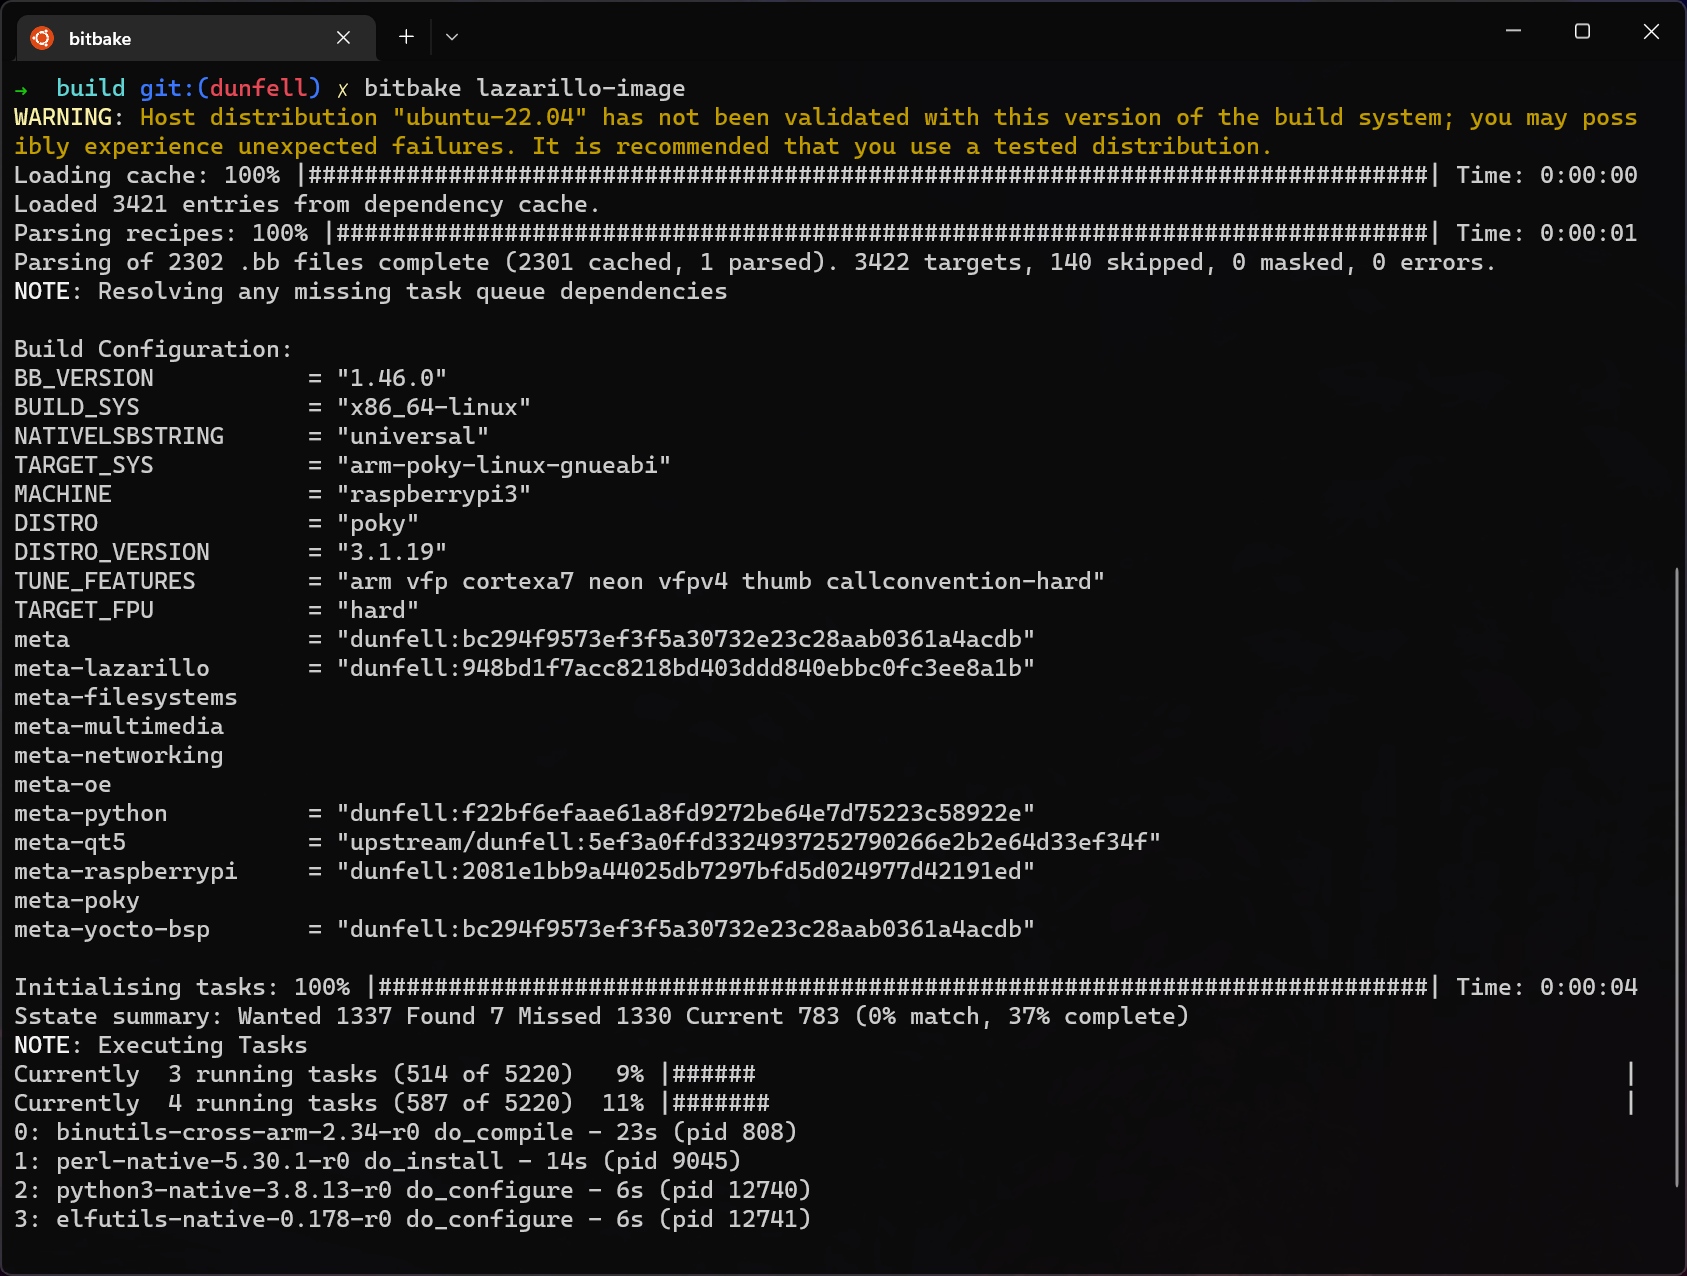
\includegraphics[width=0.95\textwidth]{imagenes/lazarillo-image-compilation.png}
	\caption{Captura de pantalla de \textit{Ubuntu 22.04} sobre el Subsistema Linux de Windows, usado para la compilación del nuevo sistema operativo.}
\end{figure}

Llegados aquí, solo quedará esperar unas horas a que termine todo el proceso. Una vez finalizado, grabaremos el archivo \textbf{\textit{lazarillo-image-raspberrypi3.sdimg}} generado bajo el directorio \emph{build/tmp/deploy/} en la tarjeta de memoria que queramos usar en el robot, la insertamos en la \textit{Raspberry} correspondiente y probamos nuestro nuevo y flamante sistema operativo personalizado.\\


\subsubsection{Personalización del sistema operativo}

Para cerrar con el sistema operativo, comentemos el caso de \textbf{\textit{psplash}} \cite{psplash}, un programa que se instala en \textbf{lazarillo-image.bb} dentro del grupo \emph{MISC\_PKGS} como dependencia externa y que permite mostrar una imagen estática durante el arranque del dispositivo final.\\

Detalles como éste hacen que el dispositivo tenga un aspecto más profesional, dado que en lugar de mostrarse una imagen genérica de \textit{GNU/Linux} o, peor si cabe, una terminal de arranque; el robot mostraría en su pantalla una imagen customizada (que podría ser un logo personalizado del proyecto, si lo hubiera).\\

Basta con integrar esta sencilla aplicación dentro del sistema operativo, cambiar la imagen que se desea mostrar y (re)compilar el sistema operativo. Sin embargo, por falta de tiempo, no he podido generar un logo personalizado para el proyecto que mostrar, por lo que el logo por defecto de \textit{OpenEmbedded} es el mostrado al iniciar.\\

\begin{figure}[h]
	\centering
	
\includegraphics[width=0.3\textwidth]{imagenes/openembedded.jpg}
	\caption{Imagen mostrada por \textit{psplash} al arranque de la máquina: logo de \textit{OpenEmbedded}, organización contribuidora activamente en el Proyecto \textit{Yocto} - Fuente: \textit{OpenEmbedded.org} \cite{openembedded}}
\end{figure}


\section{Arquitectura de Lazarillo}

Una vez que hemos visto la integración completa del sistema operativo, en esta sección enumeraremos los distintos servicios y módulos específicos creados para \textit{Lazarillo} y describiremos el propósito para el que han sido programados. Como venimos comentando, habrá ciertas partes que serán enteramente embebidas en el robot, y por otro lado también existirán otros componentes software que estarán situados ``fuera''.\\





Antes de nada, para hacernos una idea general de todos los entes involucrados en el software, prestemos atención al siguiente diagrama.\\

\begin{figure}[h]
	\centering
	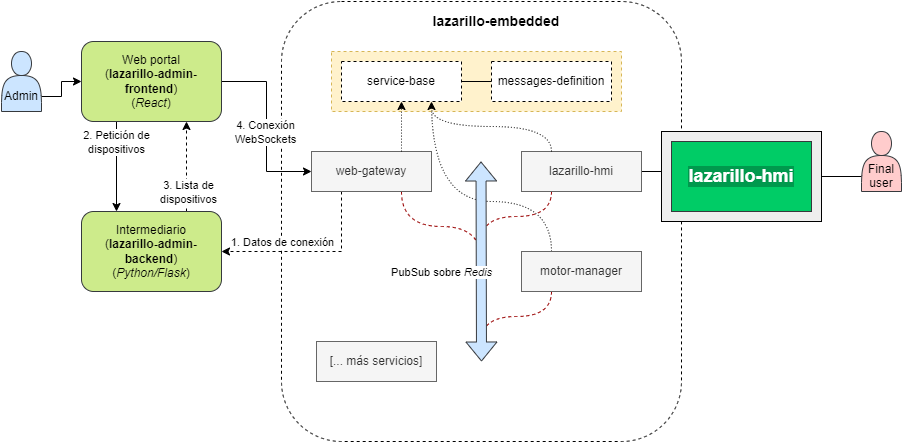
\includegraphics[width=\textwidth]{imagenes/lazarillo-architecture.png}
	\caption{Diagrama mostrando la arquitectura del proyecto, incluyendo conexiones entre servicios y relaciones internas.}
\end{figure}

\subsection{Servicios internos}

Veamos ahora una breve explicación del propósito que satisfacen los módulos software internos del robot.

\subsubsection{lazarillo-hmi}

La tecnología usada por esta aplicación, se ha decidido que sea el framework de \textbf{\textit{Qt}}, que pese a tener modalidades de licencias de pago, permite un uso \textit{open source}. Además, se trata de una tecnología con una amplia comunidad, una documentación muy rica y un gran soporte para dispositivos embebidos. Por otro lado, dispongo de amplia experiencia con dicha herramienta, lo que agiliza enormemente el tiempo de desarrollo.

Se trata de la aplicación que muestra la interfaz táctil al usuario.

\subsubsection{messages-definition}

Este módulo no es en sí un servicio sino una \textbf{librería} donde se definen los mensajes que utilizan internamente el resto de servicios para comunicarse.

\subsubsection{service-base}

Este módulo define el esqueleto abstracto de cada uno de los servicios del robot. Heredando el comportamiento de esta librería, cada uno de los nuevos servicios se ahorran procedimientos rutinarios como instanciar la conexión con la base de datos y el bróker de mensajería.

\subsubsection{web-gateway}

Este servicio es el \textit{puerto de entrada} a Lazarillo. Realiza la comunicación mediante \textit{Websockets} con \textbf{\textit{lazarillo-admin}}, el portal web a través del cual un técnico puede administrar los distintos robots. \textit{\textbf{Web-gateway}} actúa como intérprete de los mensajes provenientes del \textit{socket} y los publica en la mensajería interna del robot (basada en \textit{Redis}) para informar al resto de servicios de cualquier acción emitida por el servidor.


\subsection{Componentes externos}

Como venimos comentando, además del software embebido en el robot, disponemos de otros módulos externos a él que completan la plataforma.

\subsubsection{lazarillo-admin}

Este es el título asignado al servicio web que tanto venimos comentando a lo largo de este documento, a través del cual podemos visualizar y gestionar los distintos robots conectados al servidor.\\

Está programado con \textit{NodeJS} (TODO: ref a node) y utiliza librerías para hacer las veces de servidor con \textit{HTTPS} (para la web) y con \textit{Websockets} (para la comunicación con el robot).\\
